\section{Bacterial communities on classroom surfaces}

\subsection{Manuscript demo}

\emph{James F Meadow}\textsuperscript{1}

\textsuperscript{1} Biology and the Built Environment Center, Institute
of Ecology and Evolution, University of Oregon, Eugene, OR USA,
jfmeadow@gmail.com

\begin{center}\rule{3in}{0.4pt}\end{center}

\subsubsection{Introduction}

The data used here are a small subset (first 20,000 quality-filtered
sequences) of those previously published {[}@meadowSurfaces2014{]}. This
demo illustrates a few basic multivariate analysis methods with a sample
dataset. In the original manuscript, we investigated the sources of
microbes on classroom surfaces, and whether those microbial communities
reflect common human contact with indoor surfaces.

\subsubsection{Methods}

This sequence dataset was processed using QIIME 1.8 {[}@qiime{]} with a
default MacQIIME installation
(\url{http://www.wernerlab.org/software/macqiime}). Scripts for
processing raw data are in the \texttt{../QIIME/} folder. To pick OTUs
in that folder, you will execute the \texttt{pickTheseOTUs.sh} script
sitting in that folder. This script wants to run MacQIIME, so if you are
not using MacQIIME, you'll probably need to alter the top line to
reflect your system.

For statistical analyses, we primiarily used the \texttt{phyloseq}
package to handle QIIME output files, and \texttt{vegan} and
\texttt{labdsv} for multivariate ecology stats {[}@phyloseq; @vegan;
@labdsv{]}. All sequences were rarefied to an equal sampling depth (100
sequences per sample) prior to analysis. Beta-diversity was calculated
using the Canberra taxonomic metric. The Canberra metric is defined as:
\[ d_{jk} = \frac{1}{NZ} \sum \frac{x_{ij}-x_{ik}}{x_{ij}+x_{ik}} \]
where \emph{NZ} is the number of non-zero entries. Reproducible
documents were created with the \texttt{knitr} package in R
{[}@knitr{]}.

\subsubsection{Results}

Out of a total 1.5923 × 104 sequences that passed quality filtering, we
analyzed 5800 sequences in 58 samples distributed among 966 OTUs (97\%
sequence similarity). The most abundant OTU in the dataset was a
Cyanobacterium (2.67\% of all sequences). The most abundant taxa are
shown in Table 1. \pagebreak

\begin{table}[ht]
\centering
\begin{tabular}{rllllr}
  \hline
 & Phylum & Family & Genus & Species & RelAbu \\ 
  \hline
505954 & Cyanobacteria & Xenococcaceae & - & - & 2.67 \\ 
  1039477 & Firmicutes & Staphylococcaceae & Staphylococcus & epidermidis & 2.52 \\ 
  4449609 & Proteobacteria & Sphingomonadaceae & Sphingomonas & - & 2.40 \\ 
  359689 & Actinobacteria & Corynebacteriaceae & Corynebacterium & - & 2.16 \\ 
  4482309 & Proteobacteria & Acetobacteraceae & - & - & 2.14 \\ 
   \hline
\end{tabular}
\caption{Most abundant taxa across all surfaces.} 
\end{table}

\begin{figure}[htbp]
\centering
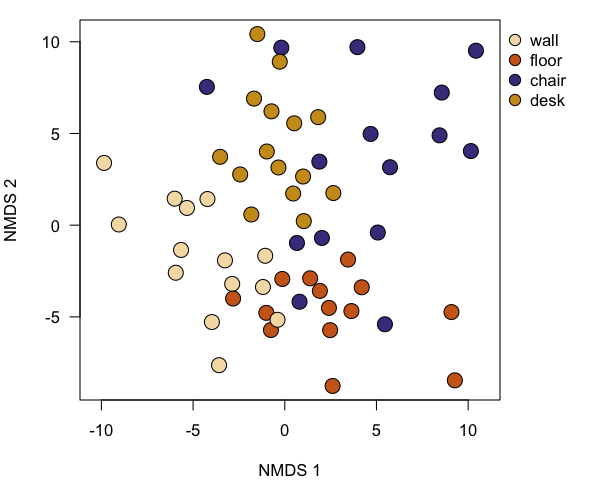
\includegraphics{figure/plotNMDS.png}
\caption{Samples cluster by the type of surface.}
\end{figure}

\begin{table}[ht]
\centering
\begin{tabular}{lrrrrrr}
  \hline
 & Df & SumsOfSqs & MeanSqs & F.Model & R2 & Pr($>$F) \\ 
  \hline
map\$SurfaceType & 3 & 2.14 & 0.71 & 1.80 & 0.09 & 0.001 \\ 
  Residuals & 54 & 21.39 & 0.40 &  & 0.91 &  \\ 
  Total & 57 & 23.52 &  &  & 1.00 &  \\ 
   \hline
\end{tabular}
\caption{Surface type explains a significant amount of variation among communities.} 
\end{table}

We found that surface type explained a significant amount of community
variation (p = 0.001; from PERMANOVA on Canberra distances).

Next, we tested for a quasi-distance-decay relationship. This is the
sort of pattern we see in just about every ecosystem with most forms of
life. We even found this to be a stong predictor in the dust sampled
from the entire building {[}@KembelPLOS2014{]}. So we can use the x and
y coordinates as a map of samples, and then calculate the Euclidean
pairwise distance between all samples. Then that goes through a mantel
test to determine if these distance are correlated with the community
distances.

We did not find any significant coorelation between community similarity
and spatial distance (p = 0.456; from Mantel test) when considering all
samples together. Likewise, individual sample types tested alone showed
no relationship with spatial distance (p \textgreater{} 0.1 for all four
sample types).

\subsubsection{Discussion}

So it looks like the type of surface, potentially as a proxy for human
contact, explains a significant amount of variation, in the microbial
communities on those surfaces, but their proximity to each other around
the room doesn't seem to matter at all.

\clearpage

\begin{center}\rule{3in}{0.4pt}\end{center}

\subsubsection{References}
